\chapter{Background}

This section highlights the key concepts that are needed to develop this project. It covers concepts including Knowledge Graphs, Natural Language Processes such as Named Entity Extraction, Sentiment Analysis, Topic Modelling that are used to extract key information from the data, understanding Word Representation as well as ways key considerations to visualise data. 

% ----------------------------------------------------------------------------------------

\section{Natural Language Pre-Processing Techniques}

First and foremost, in order to extract information (entities, relationships) from unstructured data (plain-text, e.g. news articles), the input data needs to undergo some pre-processing techniques. The combination and order of these techniques is often dependent on the use case.

Some of the most widely used pre-processing techniques in Natural Language processing include, but are not limited to, stop-word removal, tokenisation, part-of-speech (POS) tagging, normalisation (using lemmatisation and/or stemming), sentence splitting, chunking
and dependency parsing \cite{kannan2014preprocessing} \cite{ieee_named_entity}.

An example of the pipeline of showing different aspects of text preparation is as follows:

\begin{figure}[H]
\centering
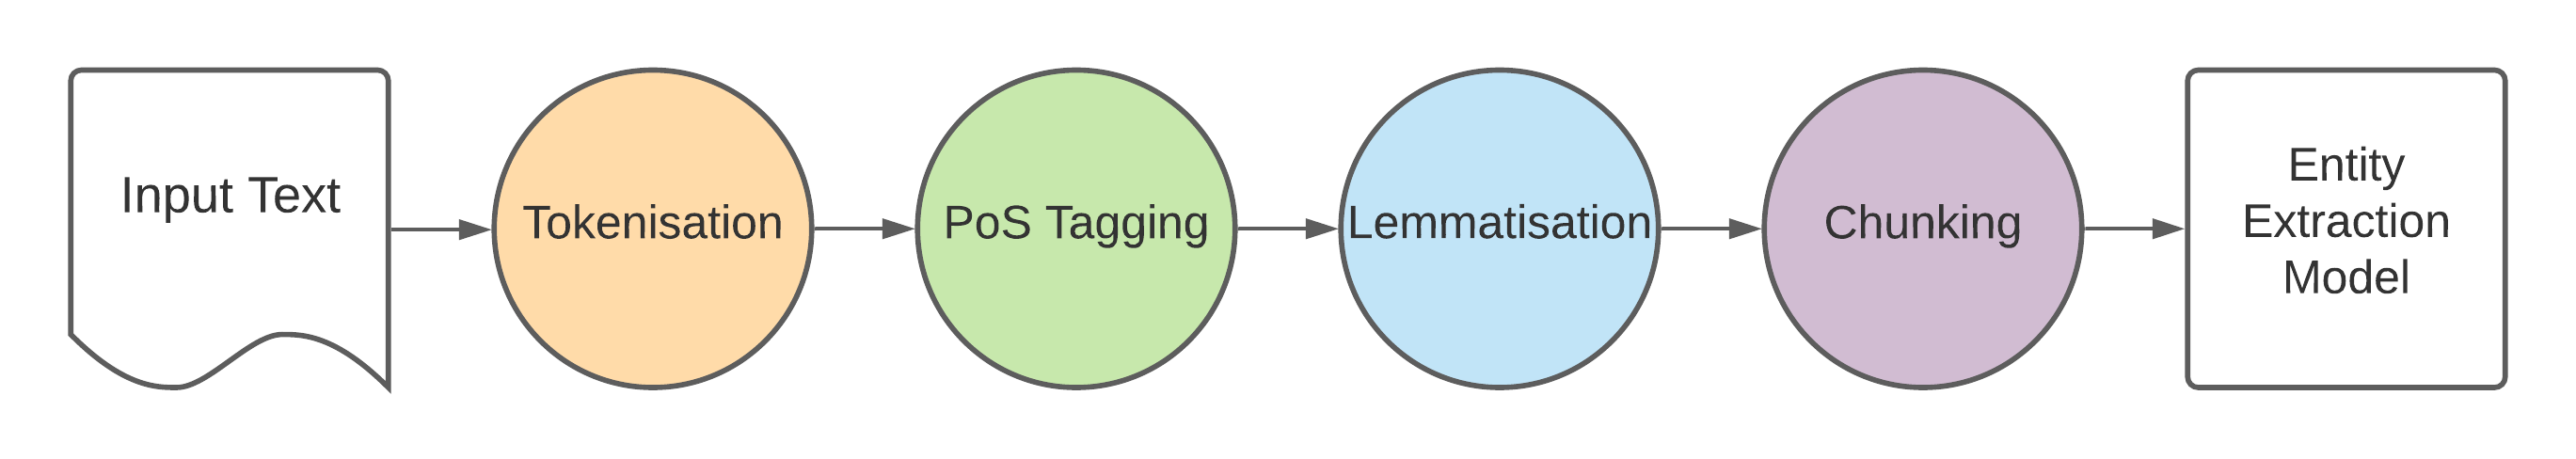
\includegraphics[scale=0.15]{images/sentence chaining}
\caption{Text preparation pipeline}
\end{figure}

\subsection{Tokenisation}
Tokenisation (as seen in Figure \ref{fig:tokenisation+pos} involves breaking down the sentence to retrieve fragments called 'tokens' which are pre-defined elements. These can include words, keywords, phrases, or symbols/ punctuation) depending on the application \cite{kannan2014preprocessing} \cite{ieee_named_entity}. Once the tokens are obtained, often some filtering methods, such as stopword removal, are applied to prune any unnecessary tokens using a pre-determined set of words (often called stoplist). This list of words is not fixed but often contains words such as 'are', 'this', 'that' etc. which are generally not crucial for document classification approaches \cite{kannan2014preprocessing}. The questions of whether stopwords should be removed and/or which stopwords to remove are often dependent on the data mining problem.  

\subsection{Part of Speech (PoS) tagging}

Part-of-speech (POS) tagging, also known as grammatical tagging, assigns 'parts-of-speech' to words in a text.  It uses word and grammar structure taking into account  the context around words to determine their characteristics, for instance, identifying a word as a noun, verb, preposition etc. \cite{pos} POS tagging often assumes some sort of tokenised text upon which it makes the grammatical tag classifications as seen in Figure \ref{fig:tokenisation+pos}. In the figure, the tagger identifies Emirates and Bitcoin as PROPN (proper nouns), airlines and payments as NOUN and as accept as VERB. POS tagging is a critical component of many NLP systems. It provides linguistic information about the text and enables information extraction from text corpora in order to identify key entities and relationships. 
% The set of tags depends on the model used and can involve course and/or fine classification. 
The set of POS tags is shown in Appendix~\Cref{appendix:pos}

\begin{figure}[H]
\centering
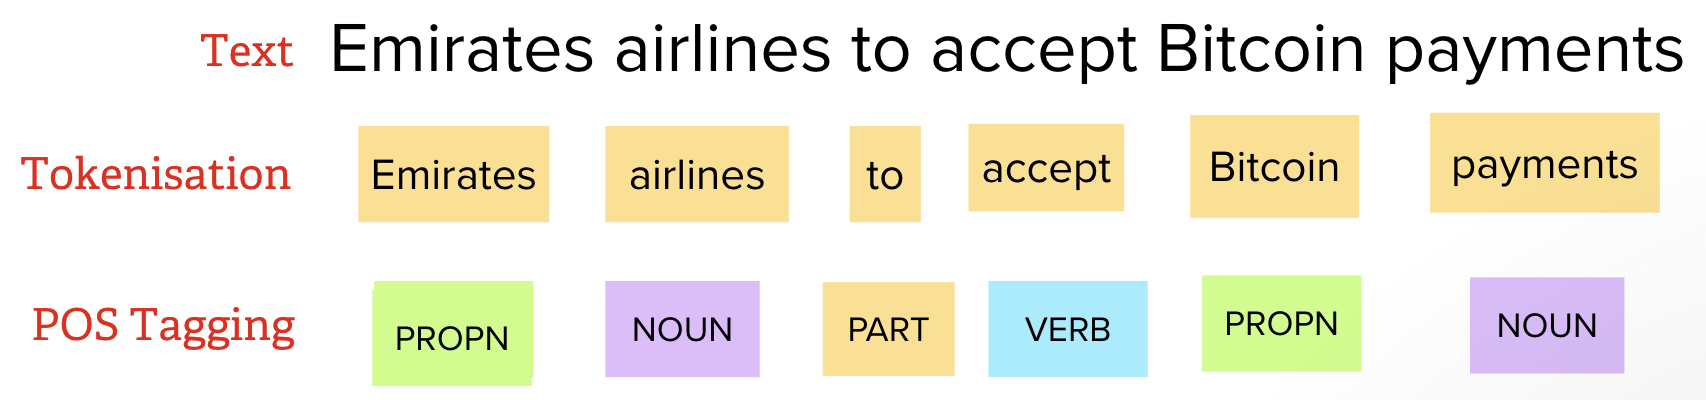
\includegraphics[scale=0.35]{images/token+pos.png}
\caption{Tokenisation and POS tagging}
\label{fig:tokenisation+pos}
\end{figure}

\subsection{Normalisation} \label{normalisation}

Information retrieval focuses on getting or
providing users with easy access to the information they need.
It does not only look for the right information but represents
it in a manner that is easily understandable to users, stores the
information in an orderly manner and organises it in such a
way that it can be easily retrieved at a later time

Normalising data is a key step in information extraction from the text. As the size of the data increases and it becomes especially important to represent data in a standard manner and reduce randomness \cite{stemming}. There are two common methods of normalising data: 

\begin{enumerate}
    \item \textbf{Stemming} is the process of reducing words (or tokens) to their word stem or root form \cite{stemming}. One of the most common algorithm for stemming english words is the Porter's algorithm. It makes use of a minimal length measure which is derived from the number of consonant‐vowel‐consonant strings that remains after a suffix is eliminated \cite{porter}. The main drawback of stemming is that it relies on a crude heuristic process to condense related words into a single stem, even if it is not a dictionary word. This can result in errors caused by under-stemming or over-stemming \cite{medium_stemming}. As an example of the latter, the words 'participation' and 'participate' may get reduced to 'participat' which is not an actual word. 
    
    \item \textbf{Lemmatisation} is a form of normalising the data by matching words with their canonical (dictionary) forms called lemmas by reducing inflictive variants to a 'root' word/token \cite{stemming}. Example: walking, walks, walked will all reduce to walk. Lemmatisation makes use of POS tags and word/ sentence structure. This is an improvement over stemming as the base words are actual words and produces much better results for language modelling as described in \cite{stemming}. 
    
\end{enumerate}

\subsection{Chunking}

Chunking is a process which essentially makes use of POS tags by attaching additional information to the sentence breaking it down into its constituent phrases. There are usually 5 major categories of extarcting chunks from text: Noun Phrase (NP), Verb phrase (VP), Adjective phrase (ADJP), Adverb phrase (ADVP) and Prepositional phrase (PP). 
For example, the sentence "The large truck is going under the tunnel" will be broken down into a noun phrase: The large truck, verb phrase: is going, prepositional phrase: under the tunnel as in Figure \ref{fig:chunking}.

\begin{figure}[H]
\centering
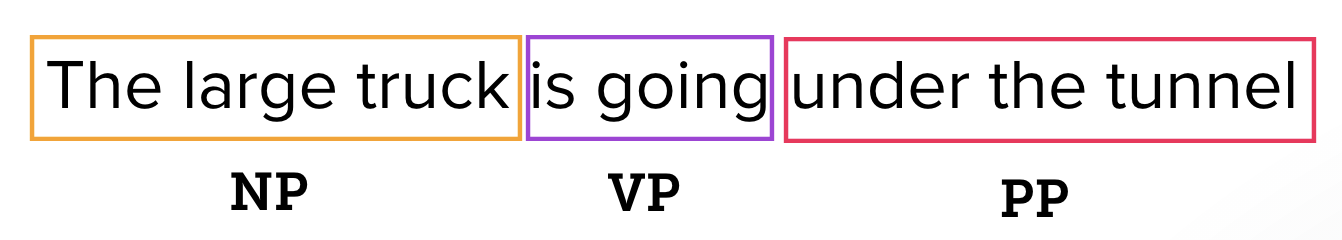
\includegraphics[scale=0.35]{images/chunking.png}
\caption{Chunking}
\label{fig:chunking}
\end{figure}



\section{Dependency Parsing} \label{dependency_grammar}
\todonum[inline, color=violet]{Write up dependency parsing}


\section{Coreference Resolution}

Coreference resolution refers to the task of ascertaining which linguistic expressions (known as mentions) in a natural language refer to the same real-world entity (such as a person or thing) \cite{zheng2011coreference}. It is often an important step for other high-level tasks such as question answering, document summarisation and information extraction. The latter use case is particularly relevant to this project. When two or more expressions, refer to the same entity, they share the same referent \cite{wiki_coref}. The goal of the coreference resolution algorithms is to find and cluster the “mentions” by their referent. For instance, in the sentence, “The U.K said they would relax travel bans”, the mentions “U.K.” and “they” refer to the same entity: U.K. 

Coreference resolution is not a trivial task as it relies on both the semantic and syntactic meaning of the text. For example, in the sentence, “Alice said she would come”, the mention “she” may or may not refer to Alice.  This indicates the complexity of the coreference resolution task as it requires contextual information, real-world knowledge, a grammatical understanding of the language etc \cite{zheng2011coreference}.

There are multiple different scenarios when exploring coreference. Some of the common ones include: 

\begin{enumerate}
    \item \textbf{Anaphora coreference: }
    Anaphoric references refer to the previous entities (the antecedent) for their meaning. For instance, in this instance “the aviation industry to find its way back in 2022”, the anaphor ‘its’ follows the expressions it refers to, the antecedent: ‘the aviation industry’. 
    
    \item \textbf{Cataphora coreference:}
    These references refer to entities/mentions later in the text. For example, in the sentence, “To aid their declining sales, Emirates is set to lower their fares”, the cataphor “their” precedes the entity/expression it refers to, the postcedent: ‘Emirates’. 
    
    \item \textbf{Split antecedents/ Multiple Antecedent Coreference:}

    These references/words have multiple antecedents that they refer to. For instance: in the sentence “British Airways and United Airlines set to resume their direct flights to Australia”, the anaphor ‘they’ has a split antecedent: ‘British Airways’ and ‘United Airlines’. 
\end{enumerate}

\subsection{Span detection}

The primary step of coreference resolution is mention detection. This involves finding the ‘spans’ i.e., the combination of words that constitute a mention. Generally, candidate spans cover NP (noun parts of the text), possessive pronouns and named entities \cite{stanfordcoref} (discussed in detail in Section \ref{named_ents}) . In order to detect spans, there are several different options for span ranking architecture. Most models are more liberal in detecting candidate spans at the initial stages and then apply some filtering and/or augmenting mechanisms to get the most relevant spans. This can involve pruning candidate spans based on a threshold ranking score, considering only a pre-determined K antecedents for each mention \cite{lee2018coursetofine} or applying the span-ranking to the text in an iterative manner to update the span representations using prior antecedent distributions to allow later coreferences to be influenced by earlier ones \cite{lee2018coursetofine}. 

\todonum[inline]{Add images:maybe}

\subsection{Coreference Architecture}
Once the candidate spans are extracted from the text, the next step is to resolve coreferences of mentions. For the purpose of this project, the most widely used architectures are focused on: 

\subsubsection{Mention-pair architecture} 
This is one of the simplest approaches and involves a binary classification task on a pair of mentions and/or entities. The classifier is given a pair of mentions, a candidate antecedent and a candidate anaphor and decides whether they are coreferring based on a score. 

\subsubsection{Mention ranking architecture}

This type of architecture directly compares the candidate antecedents with each other,  selecting the antecedent with the highest score for each anaphor. This approach is more complicated than the mention-pair model as for each anaphor, the best possible ‘gold’ antecedent is not known rather a cluster of ‘gold’ antecedents is known. In earlier models, the ‘gold’ antecedent was chosen to be the closest one. 

Generally, the simplest approach to give credit to any ‘legal’ antecedent is by adding them together and using a loss function that optimises the likelihood of all correct antecedents in the ‘gold’ cluster of antecedents \cite{stanfordcoref}. This is seen in Lee 2017 \cite{lee2017end}, \hl{a model on which a lot of recent state of the art models such} as SpanBERT \cite{spanBERT} are based on. It uses the mention ranking architecture to determine a conditional probability distribution (seen in equation \ref{cond}) to give a configuration with the highest likelihood representing the correct clustering. 

\begin{align}
 P(y_1, ..., y_n | D)  &= \prod_{i=1}^{N} P(y_i | D) \label{cond} &\\
 P(y_i) &= \frac{\exp(s(x_i, y_i))}{\sum_{y' \in Y(i)} \exp(s(x_i,y'))}  \label{coref_eq} &\\
\text{where} s(x_i,y')  &= s_m (x_i) +  s_m (y_i)  +  s_cf(x_i, y_i) \nonumber
\end{align}

In equation \ref{coref_eq}, goal of the task is to assign an antecedent to each span $x_i$ in document D. \( s(i,j)\) is a pairwise score which depends on three factors:  \(s_m(i)\), how likely span x is to be a mention; \(s_m(j)\), how likely span y is a mention and \(s_cf(i, j)\), joint coreference probability of spans i and j  in document D (assuming they are both mentions) referring to the same entity \cite{lee2017end}\cite{lee2018coursetofine}.
